\chapter[Cell Based Implicit Solvent]{A Cell Based Method for Evaluating Implicit Solvation Effects}
\label{chapter:cell_solvent}

One can see in the Generalized Born model \eqref{equation:generalized_born}, computing the electrostatic contribution to solvation requires computing the distance between every two atoms.

\section{Introduction}
\label{section:cell/intro}
% super broad computational chemistry is important because
Computational protein structure prediction and related areas of research such as target screening and lead optimization continue to be areas of active research in both pure chemistry and pharmaceutical applications \cite{jorgensen2009efficient}.
These methods range from identifying leads using chemical similarity metrics, to artificial intelligence methods such as neural networks and support vector machines, to structural based methods \cite{geppert2010current}.
In the recent past, structural methods have contributed to the identification of bioactive drug compounds \cite{corsino2009novel}, making computational protein structure prediction highly important to the medical field, and because of its pharmaceutical applications, economically relevant as well.

% the expense of computational biology and necessity of fast algorithms 
There are over 81,000 X-ray structures presently in the PDB, more than 8,500 of which have been added in the last 12 months, and the rate at which new structures are determined by X-ray crystallography continues to accelerate (see figure \ref{figure:pdb_growth}) \cite{berman2007worldwide}.
The chemical space of small molecules, i.e. potential drug compounds, is essentially unlimited, and at the least too large to effectively screen using conventional experimental methods \cite{jorgensen2009efficient}. 
Furthermore, computational loop prediction experiments are predicting longer loops, increasingly relying on the output of initial predictions as the input to a later ``fixed stage'' refinement step that re-predicts some central region of the same loop.
This has been shown to increase accuracy \cite{jacobson2004hierarchical} at the cost of an increased number of experiments and corresponding increase in computational cost.
Taken together, these factors necessitate the development of more accurate and efficient methods of generating and evaluating protein-protein and protein-small molecule conformations and interactions.

% intro of plop and solvent models
The Protein Local Optimization Program (PLOP), originally developed by Friesner and co-workers, is a popular program used to predict, sample, and evaluate protein conformations \cite{jacobson2002role,jacobson2002force,jacobson2004hierarchical}.
PLOP makes use of the OPLS-AA energy model, an atomic detail force field optimized for organic, including protein, interactions \cite{jorgensen1996development}.
In addition to the terms defined by the OPLS-AA model, it has been shown that solvent effects can make a large contribution to prediction accuracy.
The solvent contribution to an energy model can be evaluated either by explicitly modeling and sampling solvent molecules (usually water) or by treating the solvent as a continuous medium, i.e. implicit solvation.
PLOP, like many other molecular mechanics programs, makes use of an implicit solvent model.
% introduction of explicit/implicit solvent
This is largely because explicitly modeling solvent molecules, while possibly very accurate, requires extensive, and therefore very time consuming, sampling of a large number of small molecules \cite{zhang2001solvent}.
Further, energy errors using explicit solvent models can be due to either unrealistic force field parameters or insufficient sampling of solvent molecule conformations \cite{zhou2003free}.
Continuum solvation methods, or implicit solvent methods, attempt to address these issues by removing the dependence on sampling of solvent molecules and introducing approximations that reduce the cost of calculating the solvent contribution to energy \cite{roux1999implicit}.

% talking about implicit solvent
Among implicit solvent methods, the surface area based generalized Born (S-GB) model is one of the most popular and has been shown to produce results in good agreement with experimental data \cite{zhang2001solvent,gallicchio2002sgb}.
The surface area based generalized Born implicit solvent model provides an approximate solution to the Poisson--Boltzmann equation based on a surface integral \cite{ghosh1998generalized}.
However, in a naive implementation of this model, the electrostatic contribution is a sum over every charge-charge pair in the system, in this case the protein and its crystal copies.
\begin{equation}
U = \sum_{charges}U_{self}(q_k,r_k) + \sum_{charges,\ i \ne j}U_{pair}(q_i,q_j,r_i,r_j)
\end{equation}

The electrostatic contribution to solvation free energy, can be decomposed into self, and pairwise terms.
The time complexity of evaluating the pair term is quadratic in the number of charges in the system \cite{ghosh1998generalized}.
This means that calculating the electrostatic solvation contribution for a single atom requires a linear search over all other charges in the system, which for large systems becomes the bottleneck of the computation.
A common optimization is to assume that the electrostatic contribution to the solvation term for point charges separated by a distance greater than a defined cutoff distance is negligible \cite{gallicchio2004agbnp}. 
However, making this assumption does not improve the underlying quadratic time complexity of evaluating the solvation term, as it is necessary to compute the inter-charge distance for every charge pair in the system before possibly excluding the interaction.
In the implementation of S-GB in the Protein Local Optimization Program, computing the solvation term of a large structure is the rate limiting step of energy calculations, accounting for over 80\% of the total time spent computing the energy (see figure \ref{fig:timing_pie}).
Therefore, less expensive methods of evaluating the implicit solvent contribution to the energy of a system can allow for increased sampling with the same available resources, thus improving efficiency of computational modeling. 

We present an application of a geometric hashing method, grid based spatial indexing, to implicit solvent calculations in PLOP.
The hashing method proceeds by dividing space into cubical regions, or cells, and distributing atoms into those cells, while maintaining a list of the contents of each.
Retrieval of atoms within a cell can then be performed in constant time, and retrieval of a superset of atoms contained within a region can be performed in time proportional to the number of cells intersecting the region.
This efficient geometric lookup allows one to replace a loop over all atoms inside the structure with a loop over only the atoms contained in cells intersecting the sphere with radius corresponding to the distance cutoff of the force in question.
While maintaining a list of atoms for each of these grid boxes introduces some overhead when updating atomic coordinates during a simulation, updating atomic coordinate is still a constant time operation.
Thus, the benefits outweigh the costs, especially for large systems.
As long as the cell size is bounded below, the number of cells necessary to consider when evaluating a fixed distance interaction is constant.
Physical limitations provide an upper limit to atom density.
Constant time retrieval of the contents of each hash cell, along with upper bounds on the number of atoms per cell and the necessary number of cells to consider for each charge, guarantee constant time lookup of all atoms within a given sphere.
This reduces the time complexity of evaluating the electrostatic contribution from $O(n^2)$ to $O(n)$.
We show that an implementation of this hashing method can reproduce results obtained with a non-hash based implementation while providing significant performance improvements.



\section{Methods}
\label{section:cell/methods}
    \subsection{Energy Model}
    \label{subsection:energy_model}
    The energy model used in side chain prediction experiments was the optimized variable dielectric model (OVD), sometimes referenced as the variable dielectric surface generalized Born 2.0 model (VSGB2.0).
This energy model is based on the OPLS-AA energy model, which in turn gets most of its covalent parameters from the AMBER force field \cite{jorgensen1996development}.
The solvation term used is a surface area based generalized Born formulation, where the internal dielectrics of charged amino acids have been optimized over a set of 2239 single side chain predictions and 100 loop predictions of 11 to 13 residue loops.
In addition to the covalent terms from the OPLS-AA model, the current energy model also includes terms to describe $\pi-\pi$ stacking, hydrogen bonding, and a parametrized hydrophobic term for the non-polar free energy of solvation \cite{li2011vsgb}.
For the electrostatic contribution to solvation free energy, two different molecular surfaces are maintained at different resolutions.
A surface mesh is constructed for each atom using the generalized spiral points method \cite{rakhmanov1994minimal,saff1997distributing,zhou1995arrangements}.
The number of points for each sphere is 10 for the low resolution surface and 330 for the high resolution surface.
An atomic based distance cutoff is used when evaluating the electrostatic contribution to the solvation free energy.
Inside a distance of $\sqrt{50}$ angstroms, the high resolution surface is used; between this distance and 20 angstroms, the lower resolution surface is used; and the contribution of atoms outside this distance is assumed to be negligible.
The same set of cutoffs is used in both the current implementation in PLOP and the new cell based method described here.


    \subsection{Data Sets}
    \label{subsection:data_sets}
    % energy calculations data set
The data set used for energy calculation experiments consisted of large protein structures, containing neither DNA, RNA, or modified residues with molecular masses between 100 and 150 kDa. 
All samples had resolutions better than 2 angstroms. 
The data set was filtered at 30\% sequence identity, and from this, 20 structures were selected at random, though two were later excluded due to technical reasons.
% Larger structures were used to better illustrate the performance improvement using this method.

% side chain prediction data set
The structures used in side chain prediction experiments consisted of high resolution enzyme structures.
Structures without an enzyme classification were excluded, as were structures with X-ray resolution less than 1.5 angstroms, or those with modified protein residues.
This resolution requirement was imposed to make high resolution side chain prediction comparisons more meaningful.
All structures had a molecular mass between 11 kDa and 110 kDa.
Structures containing DNA, RNA or modified side chain residues were excluded, as were those that had unreasonable steric clashes either within the canonical structure or with crystal neighbors.
Structures containing certain small molecules without energy parameterizations currently defined within PLOP were also excluded.


    \subsection{Structure Preparation}
    \label{subsection:structure_preparation}
    In preparing the crystal structures for energy calculation and side chain prediction experiments, the first step was to add the crystal copies of the protein of interest.
PLOP completes this step for all space groups according to the crystal symmetry identified in the PDB file.
Before modeling a structure using an all atom force field, it is also necessary to add hydrogens and any missing heavy atoms.
When possible, PLOP uses the positions of bonded heavy atoms to build missing atoms into the structure.
However, adding hydrogens, especially for titratable residues, is a more complicated problem.
To address this, PLOP uses the independent cluster decomposition algorithm (ICDA) to determine the protonation states of any titratable residues, as well as the positions of polar hydrogens \cite{li2007assignment}.
Generally speaking, this proceeds by dividing titratable and polar residues into independent groups using a distance cutoff, and optimizing each group independently.
Structures with unreasonable steric clashes with crystal neighbors were removed from the data set on the basis that such structures are physically unlikely.


    \subsection{Grid-Based Spatial Indexing}
    \label{subsection:grid_based_indexing}
    Grid-based spatial indexing is a well known algorithm in computer science, especially computer graphics, that allows for efficient lookup based on geometric criteria and also provides fast collision detection \cite{bentley1979data}.
Critical to the present application, it allows constant time retrieval of a superset of atoms guaranteed to contain all atoms within a given Euclidean distance.
%describe when/how you set the Euclidean distance cutoff
In our implementation, the bounding box of the protein and its symmetric copies is subdivided along each of the orthogonal axes to form grid boxes or cells.
A simple convention for handling atoms that are positioned along cell boundaries guarantees that each atom is hashed to a unique cell.
For a single dimension, $d$, the cell index, or hash, of a point $p$ is 
\begin{equation}
i_{d}(p) = int\left(N * \frac{p_{d} - min_{d}(P)}{max_{d}(P) - min_{d}(P)}\right)
\end{equation}

where $min_d(P)$ and $max_d(P)$ are the minimum and maximum coordinates in dimension $d$ over the set of points $P$, $N$ is the number of cells in dimension $d$, and $p_{d}$ is the coordinate of $p$ in $d$.
Following the same procedure in each dimension gives a unique cell location for every atom.
In this way, at the beginning of the simulation, each atom is assigned to a specific cell, or grid box.
A list of the atoms in each grid box is then maintained over the course of the simulation.
When computing the electrostatic contribution to solvent free energy of an atom, $a$, it is only necessary to loop over the atoms contained in boxes that intersect the sphere corresponding to the distance cutoff around atom $a$. 
Beyond that cutoff, charge effects are considered to be negligible \cite{gallicchio2004agbnp}.
See figure \ref{figure:grid_hash} for an illustration of grid based spatial indexing in two dimensions.

In the present implementation, cell size is at first set to 2.745 angstroms, and the number of cells in a given dimension depends on the "length" of the system in that dimension.
If the number of cells that this would require is unmanageably large, cells are then grown simultaneously in all dimensions such that the cell size is 1/250th of the longest dimension of the structure.

% cells figure, pretty
\begin{figure}[h]
\begin{center}
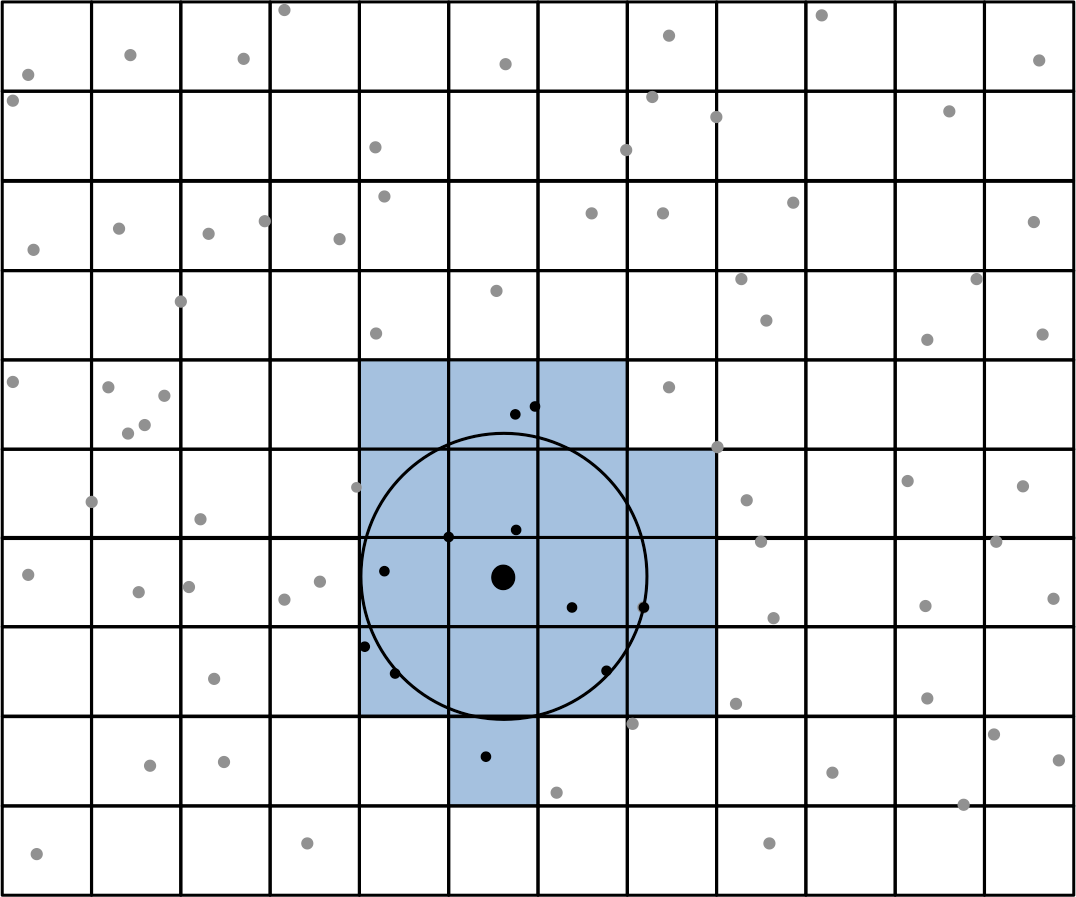
\includegraphics[width=0.6\textwidth]{figures/grid4_crop.png}
\caption{This illustrates, in two dimensions, the grid based spatial indexing method.
The naive S-GB method would require a distance computation to every other atom in the system.
By only considering atoms in cells intersecting the radius of influence, represented here in blue, it is possible to consider far fewer interactions.
Although only atoms inside the circle in this illustration contribute to surface charge, it is necessary to compute the distance over all black points.
Without using this hashing scheme, it would be necessary to compute the distance to each gray point as well.}
\label{figure:grid_hash}
\end{center}
\end{figure}


    \subsection{Experiments}
    \label{subsection:experiments}
    % side chain prediction experiments
For side chain prediction, the specific side chains used were those which had at least 30\% solvent accessible surface area when evaluated in the absence of other chains or crystal neighbors.
Glycine and proline residues were also excluded, as they do not have free side chains.
Residues missing heavy atoms in the crystal structure were predicted; however, RMSD was not measured for these residues because there is no experimental data.
Side chain prediction experiments were performed as described in \cite{jacobson2002role}.

% energy calculations experiments
The experiment in this case consisted of multiple energy calculations, using the modified version of the OPLS-AA force field described in \cite{li2011vsgb}.
In the control experiments, the same method for evaluating the implicit solvent term was used as in previous works.




\section{Results}
\label{section:cell/results}
\subsection*{Qualititave Measures of Prediction Quality}
\label{subsec:results_quality}

For side chain prediction experiments, 85.2\% of side chain prediction conformations (9406 of 11030 total) predicted with the new cell based solvation model are within 0.2 angstrom heavy atom RMSD of the prediction using the naive implementation.
In other metrics, the quality of prediction is comparable between the two solvent models. 
Median side chain heavy atom RMSD is 0.567 and 0.558 angstroms for the cell based method and the non-cell based method, respectively.
Average RMSD to the crystal structure is similarly close, 1.11 angstroms for both methods, with 79.9\% of side chain predictions within 2 angstroms RMSD of the native using the cell based model and 79.4\% within two angstroms using the naive approach.
Of side chains which are predicted differently by the two implementations there is no correlation between solvation model and prediction quality.
The distribution of side chain predictions with respect to RMSD to native is also indistinguishable between the two methods of computing the solvation term.

Data for energy calculations is not presented here because it is identical in every case.
This is expected, given that the two models represent two methods of computing the same quantity.
Thus, on the whole, prediction accuracy of the hash based model is comparable with the old implementation.

\subsection*{Performance Improvement}
\label{subsec:performance_improvement}
The principal goal of the hash based approach is to improve the performance of the implicit solvent models. 
Thus, the key metric of performance improvement is the speedup over the previous implementation.
Energy computations were found to be from 1.6 to 2.5 times as fast, and the trend indicates that even larger improvements would be obtained in larger system.
This sort of experiment represents a ``best case'' for the expected performance increase of a hash based solvent, as they represent a minimum amount of time spent on other parts of the experiment.
Implicit solvent calculations, and energy calculations in general, compose a smaller fraction of time in simultaneous side chain prediction therefore the observed performance improvement is less than that of energy calculations.
The observed performance increase in this sort of experiment is still on approximately 20\%.

\begin{figure}[H]
\begin{center}
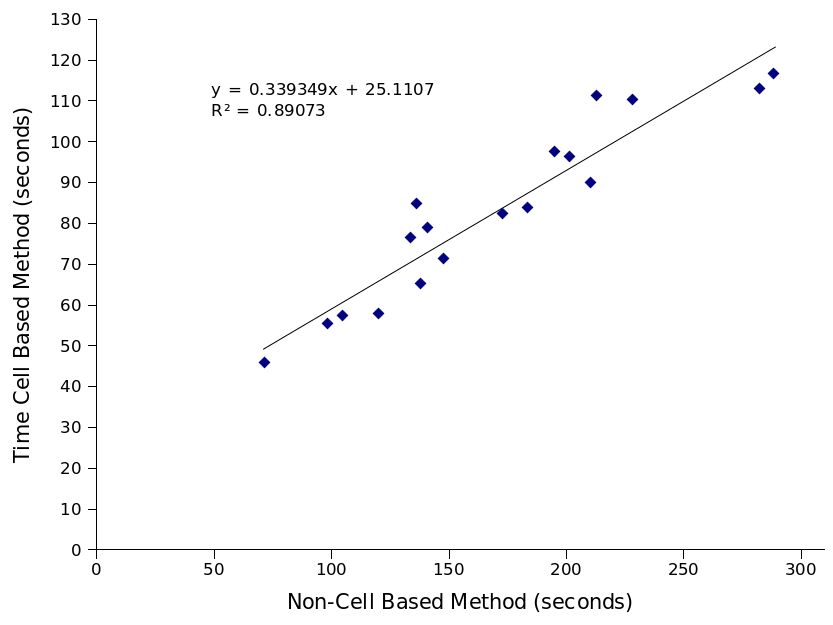
\includegraphics[width=0.8\textwidth]{figures/energy_calculation_timings.png}
\caption{Energy computations using a grid based method yields approximately a three times performance improvement, though in the case of some very small structures it is possible that the overhead introduced by maintaining the grid structure outweighs the improvement.}
\label{fig:ddr}
\end{center}
\end{figure}

\begin{table}[H]
\centering
\label{table:energy_timings}
\begin{tabular}{|c|c|c|}
\hline
PDB id	& Naive Method	& Cell Based Method	\\
\hline
1F5Z	&   201.75	&   96.37	\\
1H2V	&   98.31	&   55.32	\\
1HRD	&   228.38	&   110.12	\\
1M1Z	&   147.83	&   71.28	\\
1M9X	&   282.35	&   113.04	\\
1O60	&   172.82	&   82.34	\\
1R0V	&   210.35	&   90.0    \\
1XMP	&   213.25	&   111.25	\\
2E3Z	&   141.11	&   78.79	\\
2H6U	&   138.25	&   65.07	\\
2OU1	&   104.93	&   57.24	\\
2XI9	&   71.68	&   45.73	\\
3AMD	&   288.58	&   116.52	\\
3DEL	&   133.62	&   76.48	\\
3E1E	&   183.8	&   83.8	\\
3FGN	&   120.38	&   57.75	\\
3HHP	&   195.25	&   97.58	\\
4GVR	&   136.35	&   84.78	\\
\hline
\end{tabular}
\caption{The specific timings for a series of energy computations presented in Figure \ref{fig:ddr}.
These represent a ``best case'' scenario, as the majority of time in these experiments is spent computing the solvent contribution.}
\end{table}
% Would it be useful in this table to add a column that shows %improvement?






\section{Discussion}
\label{section:cell/discussion}
%Summarize what you did and results
We have developed an application of a classic computer science grid based hashing algorithm to the implicit solvent model of PLOP.
We demonstrate that this application does not affect accuracy of results compared with the previous implicit solvent model implementation in PLOP.
Though in a small number of cases side chain conformations are predicted in widely different conformations by the hash based method and the old implementation, the two methods are equally likely to predict the more native-like structure, so this variance can be attributed to noise.
We have also found in other experiments that the final predicted structure of a minimization is very sensitive to both small changes in pre-minimization coordinates, of a magnitude far less than bond distances, and minimization parameters.
It possible that these effects magnify small differences present early in the experiment, resulting in much larger differences between the final predicted structures.
Finally, we present data showing that the reduced computational cost of evaluating the solvent contribution using this hash based approach dramatically reduces the total time spent evaluating the energy model by a factor of 1.6 to 2.5.

% talk about hash method, 
Note that any such geometric hashing will introduce some overhead for maintaining the data structure.
As discussed by Bentley and Friedman \cite{bentley1979data}, the total storage necessary for the hash structure and the time necessary to sort atoms into cells are both linear in the number of atoms, and placing or updating a single atom in the structure is a constant time operation.
The improvement in retrieval using this structure dominates the cost of maintaining the structure, and the difference becomes more pronounced as system size grows.
Bentley and Friedman also present a through review of the performance characteristics of a number of other geometric hashing techniques, though they compare the algorithms in a data agnostic means.
Taking advantage of the characteristics of physical data, in this case atomic coordinates, has some effect of the relative advantages and disadvantages of specific hashing techniques. 
Specifically, the maximum number of atoms per cell is limited by physical constraints of atomic interactions.
% other hashing methods - octree.  why yours is better
An octree is a similar, though hierarchical, hash structure used in computer graphics for fast location based retrieval.
However, because the criteria for ``collision'' in this case is a fixed distance cutoff, and the data is roughly uniformly distributed it is efficient to used a fixed cell size\cite{turk1989interactive}.

% Can be implemented anywhere there is a pair interaction term
Though the implicit solvent term was initially targeted, because it dominates the time spent in energy calculations, it is possible to apply this method to any pair-pair interaction.
Though especially for shorter range interactions it might be beneficial to either maintain a higher resolution hash, or implement a hierarchical spatial hash, such as an octree.
We are also applying this geometric hashing technique to collision detection between simultaneous loop predictions.
This will allow efficient screening of neighboring loop prediction candidates, which will be particularly useful in predicting structures with multiple nearby solvent exposed loops, such as G-protein coupled receptors.

% implicit/explicit comparison discussion
Implicit solvation models offer a very tangible benefit over explicit solvent models, both in performance and experimental complexity.
Though explicit solvation is sometimes viewed as a ``gold standard'', it has been shown that current implicit solvent models can, at least sometimes, reproduce predictions of explicit solvent models.
However, development of implicit solvent models is important since improved performance compared with explicit solvent methods allows modeling of larger systems, longer timescales, or improved sampling.
The complexity of the experiment is also reduced, using implicit solvent models, because results are not dependent on sampling of water conformations in addition to protein conformations.
However, implicit solvent models can still be very computationally expensive.
For instance, in the PLOP implementation of the OPLS-AA energy model with SG-B solvation term, evaluating the solvation term consumes up to 80\% of the total time spent in energy calculations, dependent on size of the symmetric system.
This is in large part due to the time complexity of evaluating the SG-B solvation term.
Thus an algorithm that offers further reduction in experimental cost without a tradeoff in accuracy represents valuable progress in the development of implicit solvent models.


%%%%%%%%%%%%%%%%%%%%%%%%%%%%%%%%%%%%%%%%%%%%%%%%%%%%%%%%%%%

% practical considerations and limitations
Because the size of protein systems are limited, at some level, by physical limits, the maximum system size expected to be encountered is limited.
Therefore, although the new method reduces the time complexity of implicit solvent calculations, the maximum expected speedup is limited to about a factor of three in large systems.
The actual speedup depends on both the system size, and the amount of time that a given experiment spends evaluating the solvent contribution.
The speedup observed in side chain prediction experiments was much less, around 20\%, though it is possible that applying a similar method to terms of the gradient during minimization would increase that amount.
Nonetheless, even a 20\%  speedup represents a significant improvement, especially as structure prediction methods continue to depend on parallel prediction and reprediction of the same region as a method of structure refinement\cite{goldfeld2013loop}.
% could be future work
Although this algorithm improves on the theoretical time complexity of the S-GB implicit solvent model, parameterization such as the number, and size of cells in the grid structure could have a significant effect on run time.
Some effort was made towards choosing reasonable parameters, but they are likely not optimal.
Hardware that is optimized for this sort of spatial indexing and collision detection, or proximity detection, exists in modern video cards, and along with general purpose programming for this sort of hardware it should be possible to further parallelize computation of implicit solvation effects for even greater performance improvements\cite{harris2008cuda}.

\subsection*{Acknowledgements}
\label{subsec:acknowledgements}
Experiments were performed by J.B. over the last year at the Columbia University Chemistry Department cluster on a mix of hardware. 
J.B. is funded by XXXX.
R.F. is funded by XXXX. R.F. has a significant financial stake in Schr\"{o}dinger, Inc., is a consultant to Schr\"{o}dinger, Inc., and is on the Scientific Advisory Board of Schr\"{o}dinger, Inc.


